\documentclass[12pt]{beamer}
\usetheme{Boadilla}
\usecolortheme{dolphin}
\usepackage{hyperref}
\usepackage{tikz}
\usepackage{algorithm}
\usepackage{algpseudocode}

\newcommand{\myTitle}{\rmfamily\bfseries}

\title[AD equation solver based on Allscale API]{
\myTitle Data Assimilation For Advection-Diffusion Flows By Interconnected Localized Filters: \\ a case study of Allscale API}
\author[IBM Research Ireland 2017]
{{\small Emanuele Ragnoli,  Fearghal O'Donncha,  Albert Akhriev} \\ \vspace{0.5em}{\large IBM Research Ireland}}

% Insert frame number.
%\expandafter\def\expandafter\insertshorttitle\expandafter{%
%\insertshorttitle\hfil\insertframenumber\,/\,\inserttotalframenumber}

\begin{document}

\begin{frame}
\maketitle
\end{frame}

\begin{frame}{\myTitle The Problem}
\begin{itemize}
\item An oil spill is the release of a liquid petroleum hydrocarbon into the environment, which is unfortunate but possible event.
\item Marine fauna is especially vulnerable.
\item Monitoring oil contamination over time in the affected area is an important part of clean up operation.
\item Assuming that the level of pollution can measured at some locations within contaminated region (e.g. by remote sensing), the process of spreading the oil can be described by the well-known physical model.
\end{itemize}
\end{frame}

\begin{frame}{\myTitle The Model}
\begin{itemize}
\item The equation for the process of substance (oil) dissemination driven by two physical phenomena -- advection and diffusion:   
$$
\frac{\partial u}{\partial t} = 
D \left( \frac{\partial^2 u}{\partial x^2} +  \frac{\partial^2 u}{\partial y^2} \right)
- v_x \frac{\partial u}{\partial x} - v_y \frac{\partial u}{\partial y} + f(x,y,t),
$$
where $u = u(x,y,t)$ is oil concentration, $D$ is diffusion coefficient, $(v_x, v_y)$ are components of flow velocity, and $f$ is contamination source term.
\item In simplified set-up $D$ is a constant, $(v_x, v_y)$ depend on time only, $f$ is a high concentration spot at  $t=0$ around one point and zero elsewhere, and $u(\Gamma)$ = $\frac{\partial u(\Gamma)}{\partial {\bf n}}$ = 0 on the boundary $\Gamma$ of the domain $\Omega$.
\end{itemize}
\end{frame}

\begin{frame}{\myTitle Data Assimilation}
\begin{itemize}
\item Observations are available at few points of the domain Ω. 
\item In order to obtain full picture of oil dispensing, the information should be spread from observation points to their unobservable neighbours.
\item The information propagation is achieved by means of Kalman filtering.
\item Kalman filter updates a (sub-)domain field of contaminant distribution utilizing information at observation points (sensors). 
\item Filtering drags the simulation process (which starts from zero field) towards the “true” state of the nature provided by measurements.
\end{itemize}
\end{frame}

\begin{frame}{\myTitle Computational Problem}
\begin{itemize}
\item Had it been applied to the whole domain $\Omega$, the Kalman filter would be prohibitively expensive as it comprises inversion of a dense matrix ($O(N^3)$).
\item Also, the higher resolution (the larger problem size $N$) -- the smaller time step (the larger number of iterations) is needed to satisfy the CFL condition. As such, each step should be fast enough to make reasonable computation time.
\end{itemize}
\end{frame}

\begin{frame}{\myTitle Domain sub-division}
\begin{itemize}
\item Dividing the domain into sub-domains is a common circumvention to the large computational problems.
\item Allscale API provides advanced facilities for domain partitioning and parallel framework for efficient solving a set of smaller sub-problems.
\item In Amdados application we solve a number of sub-problems in parallel and independently.
\item In order to approximate the global solution, a variant of Schwarz method iteratively refines the solution by exchanging the information at sub-domain boundaries, which is a relatively cheap operation. 
\end{itemize}
\end{frame}

%\begin{algorithmic}[1]
%	\State set property field at the lowest resolution;
%	\Repeat
%	\State minimize misfit given property field;
%	\State increase resolution by a certain factor;
%	\Until{(resolution = finest resolution)}
%\end{algorithmic}

\begin{frame}{\myTitle Amdados application}
\begin{itemize}
\item Solves the data assimilation problem based on advection-diffusion equation.
\item Demonstrates the power of Allscale API in solving the challenging real world problems.
\item Currently implements an implicit advection-diffusion solver based om finite-difference discretization applied to a sub-domain.
\item The global solution is refined by Kalman filtering coupled with Schwarz method that exchanges the information at the sub-domain boundaries.
\item More advanced approaches (FEM, Minimax filtering) are currently investigated and partially implemented. 
\end{itemize}
\end{frame}

\begin{frame}{\myTitle Amdados:  the observations}
\begin{itemize}
\item In practice, the true state of the nature is available at a (small) subset of domain points where the sensors can measure the concentration.
\item In our demo, the measurements (aka “analytic solution”) are synthesized by the global implicit forward solver written in Python3.
\item The solver does not do domain decomposition (having limited scalability) and does not apply any filtering – just forward time-marching of advection-diffusion PDE.
\item The solution at each time step is recorded into the file of observations and used in simulation as the “sensor measurements”.
\end{itemize}
\end{frame}

\begin{frame}{\myTitle Amdados: the measurements}
\begin{columns}[c, onlytextwidth]     %EVEN SPECIFYING THE c OPTION
\begin{column}{.33\textwidth}%
\setlength{\partopsep}{0pt}                %AND EVEN REMOVING EXTRA itemize SPACE
{\small \begin{itemize}
%\itemsep 1.5em
\item The ``sensors'' are seeded randomly inside each sub-domain.
\item Only observations at the “sensor” locations are used during simulation.
\item White dots show ``sensors''; gray lines outline the sub-domain borders.
\end{itemize}}
\end{column}%
\begin{column}{.75\textwidth}
\begin{center}
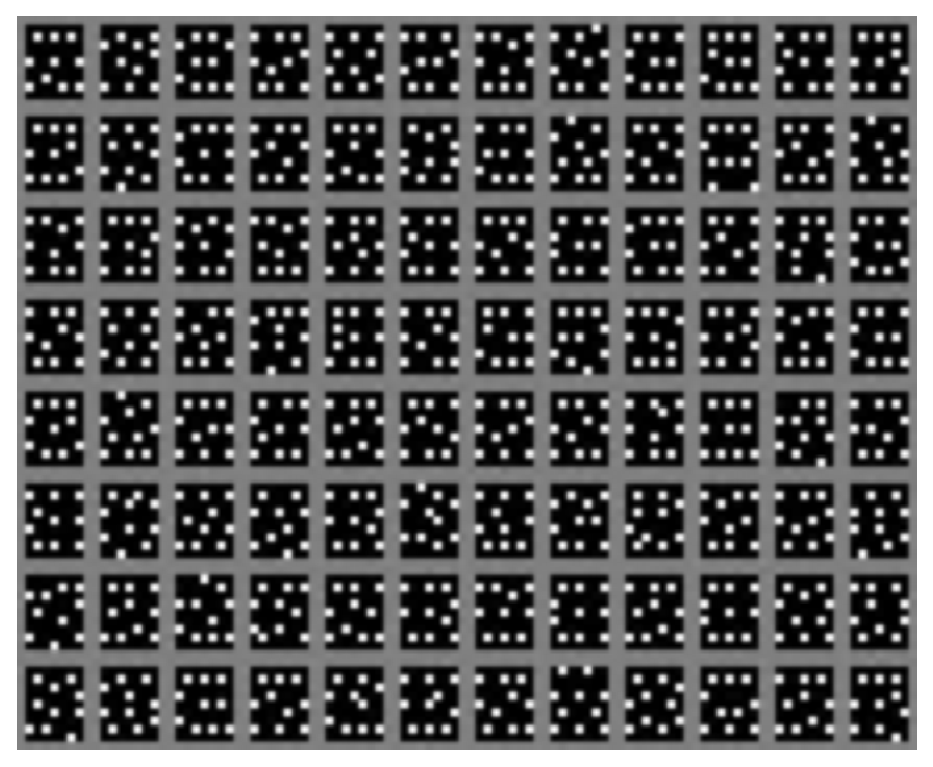
\includegraphics[width=0.8\textwidth,keepaspectratio]{images/sensors-small.eps}
\end{center}
\end{column}%
\end{columns}
\end{frame}

\begin{frame}{\myTitle Example: sensors in high resolution}

\includegraphics[width=\textwidth,keepaspectratio]{images/sensors-big.eps}
\end{frame}

\begin{frame}{\myTitle Amdados: the simulation}
\begin{itemize}
\item The goal is to synthesize contamination distribution inside the domain given measurements of the ``true'' field at a (small) sub-set of points where ``sensors'' are located.
\item We start with zero field at $t=0$ because the true state of nature is not known in advance.
\item Gradually, the Kalman filter integrated with Schwarz method (for exchanging the information across sub-domain borders) makes the simulated field look quite similar the true one.
\item In this way, a reasonable estimation of contamination level can be done in unobserved domain points on each time step.
\end{itemize}
\end{frame}

\begin{frame}{\myTitle Amdados: Kalman filter}
\begin{itemize}
\item \textit{Process model}: ${\bf x}_{t+1} = {\bf A}{\bf x}_t + {\bf w}_t$,  where ${\bf x}$ is the state field (space distribution of contaminant), ${\bf A}$ is the model matrix (finite-difference discretization) and ${\bf w}$ is the process noise.
\item \textit{Implicit method}:  ${\bf B}{\bf x}_{t+1} = {\bf x}_t + {\bf\tilde w}_t$, ${\bf B} = {\bf A}^{-1}$.
\item \textit{Measurement residual}: ${\bf y}_t = {\bf z}_t - {\bf H}{\bf x}_t$ where ${\bf z}$ is the vector of observations at sensor locations, ${\bf H}$ is a low-rank observation matrix.
\item \textit{Prior state estimation}:  ${\bf\hat x}_{t+1} = {\bf A}{\bf x}_t$,  ${\bf\hat P}_{t+1}  = {\bf A}_t {\bf P}_t {\bf A}_t^T + {\bf Q}_t$,  where ${\bf P}$ is the process covariance matrix and ${\bf Q}$ is the process noise covariance.
\item \textit{Posterior estimation}:  ${\bf x}_{t+1} = {\bf\hat x}_{t+1} + {\bf K}_t {\bf y}_t$ ,  ${\bf P}_{t+1} = ({\bf I} - {\bf K}_t {\bf H}_t) {\bf\hat P}_{t+1}$ where ${\bf K}$ is the Kalman gain matrix.
\item Several posterior estimation steps are consecutively repeated in Schwarz method until sub-domain fields match at borders.
\end{itemize}
\end{frame}

\begin{frame}{\myTitle Amdados: Schwarz iterations}
\begin{itemize}
\item Each sub-problem is propagated forward in time independently. As such, new estimations can significantly disagree along sub-domain borders.
\item The Schwarz method solves a boundary value problem for a PDE approximately by splitting it into boundary value problems on smaller domains and iteratively combining the results. We use adaptive AND/ARN variant by Gastaldi et al., 1998.
\item If flow coming into a sub-domain across a border (Up, Down, Left or Right), the border values of the neighbor sub-domain replace the corresponding border values of this one.
\item If flow going out of the sub-domain, the Neumann conditions are imposed on the respective border.
\end{itemize}
\end{frame}

\begin{frame}{\myTitle Amdados: the algorithm}
\begin{algorithmic}[1]
\State Start from zero field ${\bf x}_0 = 0$ and near-identity covariance ${\bf P}_0 \sim {\bf I}$. 
\For {t = 0:$N_t$}
	\State Propagate state one step ahead ${\bf\hat x}_{t+1}$, ${\bf\hat P}_{t+1}$.
	\State Get observation vector ${\bf z}_t$.
	\For {t = 1:$N_{schwarz}$}
		\State Get posteriors ${\bf x}_{t+1}$, ${\bf P}_{t+1}$ by solving Kalman filter.
		\State Apply Schwarz update.
		\State Apply boundary conditions at the global border. 
	\EndFor
	\State Replace by the last posteriors: $\{{\bf x}_t, {\bf P}_t\}$ $\leftarrow$ $\{{\bf x}_{t+1}, {\bf P}_{t+1}\}$.
	\State $t \leftarrow t + 1$
\EndFor
\end{algorithmic}
\vspace{1em}
N O T E: \textbf{fixed} number of Schwarz iterations -- global reduction is discouraged by Allscale API.
\end{frame}

\begin{frame}{\myTitle Schwarz iterations: relative error}
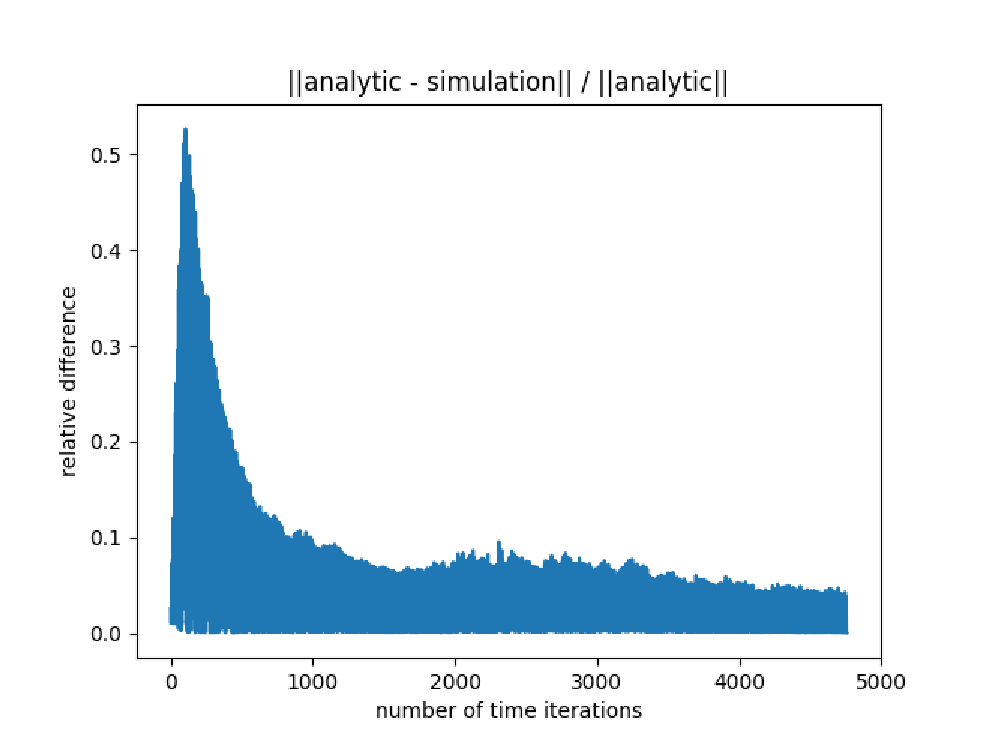
\includegraphics[height=0.9\textheight,keepaspectratio]{images/schwarz-diff.eps}
\end{frame}

\begin{frame}{\myTitle Closer look at the relative error}
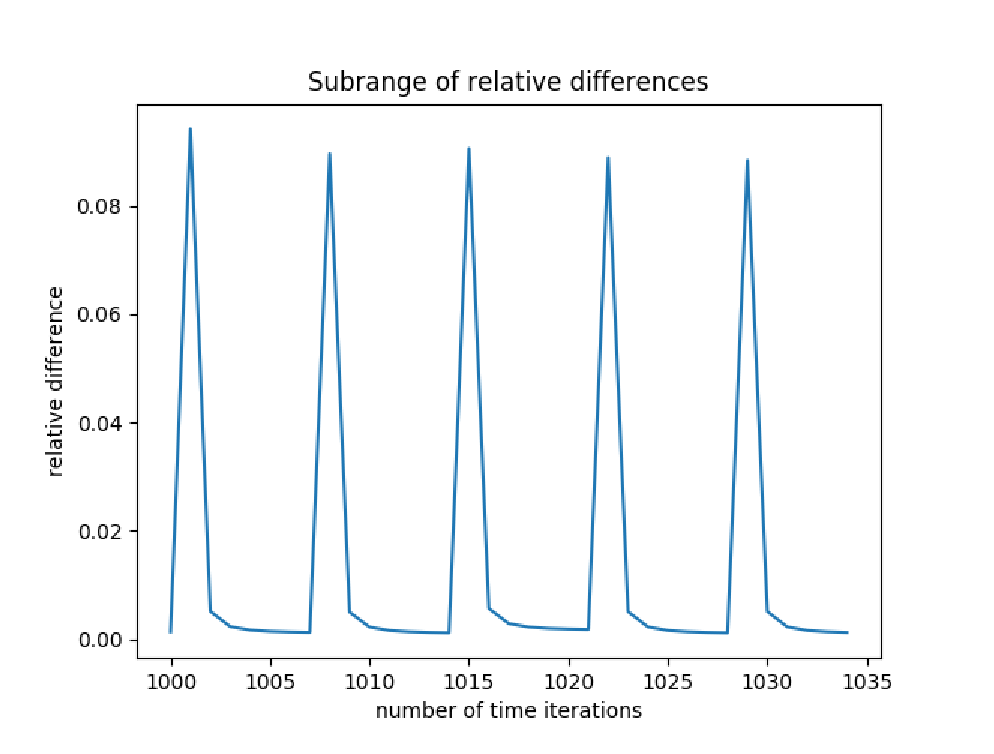
\includegraphics[height=0.9\textheight,keepaspectratio]{images/schwarz-diff-subrange.eps}
\end{frame}

\begin{frame}{}
\centerline{\LARGE \bf Thank You!}
\end{frame}

\end{document}
